\documentclass[12pt,xcolor=dvipsnames]{article}
\usepackage[utf8]{inputenc}
\usepackage[vietnamese]{babel}
\usepackage{amstext,latexsym,amsbsy,amssymb,amsmath,amsthm,amsfonts,exscale,eucal}
\usepackage{appendix}
\usepackage{algorithm}
\usepackage{graphicx}
\usepackage{xcolor}
\usepackage{hyperref}
\usepackage{indentfirst}
\usepackage{enumitem}
\usepackage{diagbox}
\usepackage{booktabs}

\usepackage[left=2.00cm, right=2.00cm, top=2.00cm, bottom=2.00cm]{geometry}
\setlength{\parskip}{5pt}%khoảng cách dòng
\renewcommand{\baselinestretch}{1.15}
\theoremstyle{definition}
\newtheorem{vd}{Ví dụ}[section]
\newtheorem*{giai}{Giải}
\newtheorem{bt}{Bài tập}
\renewcommand{\l}{\left}
\renewcommand{\r}{\right}
\date{}

\begin{document}
\begin{bt}
Dữ liệu \texttt{mars.dat} cung cấp dữ liệu về hồ sơ nhiệt độ-áp suất của khí quyển sao Hỏa, được tàu vũ trụ Mars Global Surveyor đo vào năm 2003 bằng kỹ thuật che khuất sóng vô tuyến. Nhiệt độ (temperatures) nhìn chung giảm khi bán kính (radius) tâm hành tinh (độ cao) tăng.

\begin{enumerate}[label=(\alph*)]
    \item Áp dụng hàm đã làm trong câu 3 để làm dự đoán xu hướng thay đổi của nhiệt độ theo bán kính tâm hành tinh thay đổi.
    \item Dữ liệu này bắt nguồn từ bảy quỹ đạo riêng biệt của tàu vũ trụ. Các quỹ đạo này đi qua các vùng hơi khác nhau của sao Hỏa. Một tập dữ liệu đầy đủ hơn bao gồm số quỹ đạo, áp suất khí quyển, kinh độ, vĩ độ và các biến khác có sẵn trong tệp \texttt{marsbig.dat}. Hãy xác định xu hướng thay đổi của nhiệt độ theo bán kính tâm hành tinh khi tàu vũ trụ bay trong các quỹ đạo (orbit) khác nhau.
    \item Trong trường hợp thay thế bán kính (radius) bằng áp suất (pressure) thì xu hướng thay đổi của nhiệt độ là như thế nào?
\end{enumerate}
\end{bt}

\begin{giai}

\textbf{Mô tả dữ liệu}

Dữ liệu \texttt{mars.dat} chứa 80 quan sát với 3 biến:
\begin{itemize}
    \item \texttt{radius}: Bán kính tâm hành tinh (km), tương ứng với độ cao trong khí quyển
    \item \texttt{temperature}: Nhiệt độ khí quyển (K - Kelvin)
    \item \texttt{sigmatemperature}: Sai số đo lường nhiệt độ
\end{itemize}

Dữ liệu \texttt{marsbig.dat} chứa 324 quan sát với 11 biến, bao gồm thêm: \texttt{latitude}, \texttt{longitude}, \texttt{pressure}, \texttt{orbit}, và các biến khác.

\textbf{Phương pháp}

Sử dụng hàm \texttt{locpoly\_reg()} từ Bài tập 3 với các bậc đa thức:
\begin{itemize}
    \item $p=0$: Nadaraya-Watson (local constant)
    \item $p=1$: Local linear regression
    \item $p=2$: Local quadratic regression
\end{itemize}

Băng thông $h$ được chọn tự động qua Leave-One-Out Cross-Validation (LOOCV).

%=============================================================================
\subsection*{Phần (a): Xu hướng nhiệt độ theo bán kính}

Áp dụng hồi quy đa thức cục bộ cho dữ liệu \texttt{mars.dat} với biến độc lập $X = \texttt{radius}$ và biến phụ thuộc $Y = \texttt{temperature}$.

\textbf{Kết quả bandwidth tối ưu:}
\begin{center}
\begin{tabular}{lcc}
\toprule
Bậc đa thức & Bandwidth $h$ (km) & CV Score \\
\midrule
$p=0$ (Nadaraya-Watson) & 1.4031 & 6.7352 \\
$p=1$ (Local Linear) & 1.8204 & 6.6688 \\
$p=2$ (Local Quadratic) & 4.6304 & 6.6214 \\
\bottomrule
\end{tabular}
\end{center}

\textbf{Phân tích xu hướng:}

Kết quả cho thấy nhiệt độ \textbf{giảm} khi bán kính (độ cao) \textbf{tăng}:
\begin{align}
\frac{\partial \hat{m}(x)}{\partial x} \approx -0.61 \text{ K/km}
\end{align}

Điều này phù hợp với đặc điểm khí quyển sao Hỏa: càng lên cao (radius lớn), nhiệt độ càng giảm, tương tự hiện tượng trong tầng đối lưu của Trái Đất.

\begin{figure}[h]
\centering
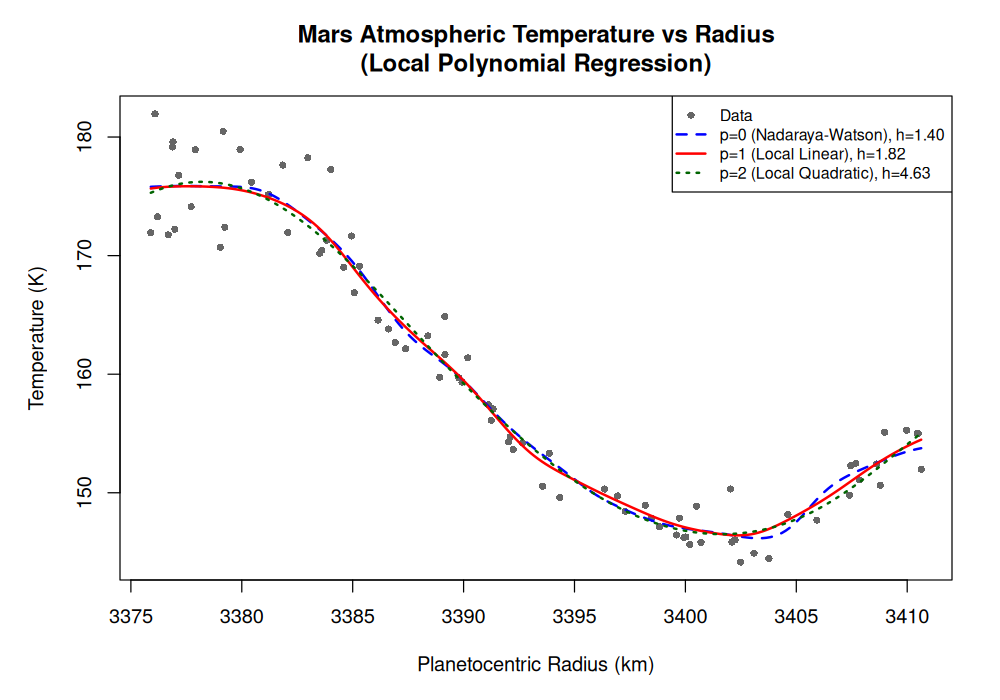
\includegraphics[width=0.8\textwidth]{exercise_04a_temp_vs_radius.png}
\caption{Nhiệt độ khí quyển sao Hỏa theo bán kính tâm hành tinh}
\end{figure}

%=============================================================================
\subsection*{Phần (b): Phân tích theo từng quỹ đạo}

Dữ liệu \texttt{marsbig.dat} được chia theo 7 quỹ đạo riêng biệt. Mỗi quỹ đạo đi qua các vùng kinh độ khác nhau của sao Hỏa (vĩ độ tương đối ổn định $\approx 71.5^\circ$ Bắc).

\textbf{Kết quả phân tích theo từng quỹ đạo:}
\begin{center}
\begin{tabular}{cccc}
\toprule
Quỹ đạo & Số quan sát & Bandwidth $h$ (km) & Độ dốc (K/km) \\
\midrule
1 & 46 & 1.4771 & $-0.4904$ \\
2 & 46 & 1.5037 & $-0.7556$ \\
3 & 47 & 1.4903 & $-0.7044$ \\
4 & 47 & 1.4995 & $-0.6977$ \\
5 & 46 & 1.4864 & $-0.6844$ \\
6 & 46 & 1.5141 & $-0.6612$ \\
7 & 46 & 1.4678 & $-0.6221$ \\
\bottomrule
\end{tabular}
\end{center}

\textbf{Nhận xét:}
\begin{itemize}
    \item Tất cả 7 quỹ đạo đều cho thấy xu hướng \textbf{giảm} tương tự (độ dốc âm).
    \item Độ dốc dao động từ $-0.49$ đến $-0.76$ K/km.
    \item Sự khác biệt nhỏ giữa các quỹ đạo do đi qua các vùng kinh độ khác nhau của sao Hỏa.
    \item Kết quả xác nhận xu hướng chung của phần (a).
\end{itemize}

\begin{figure}[h]
\centering
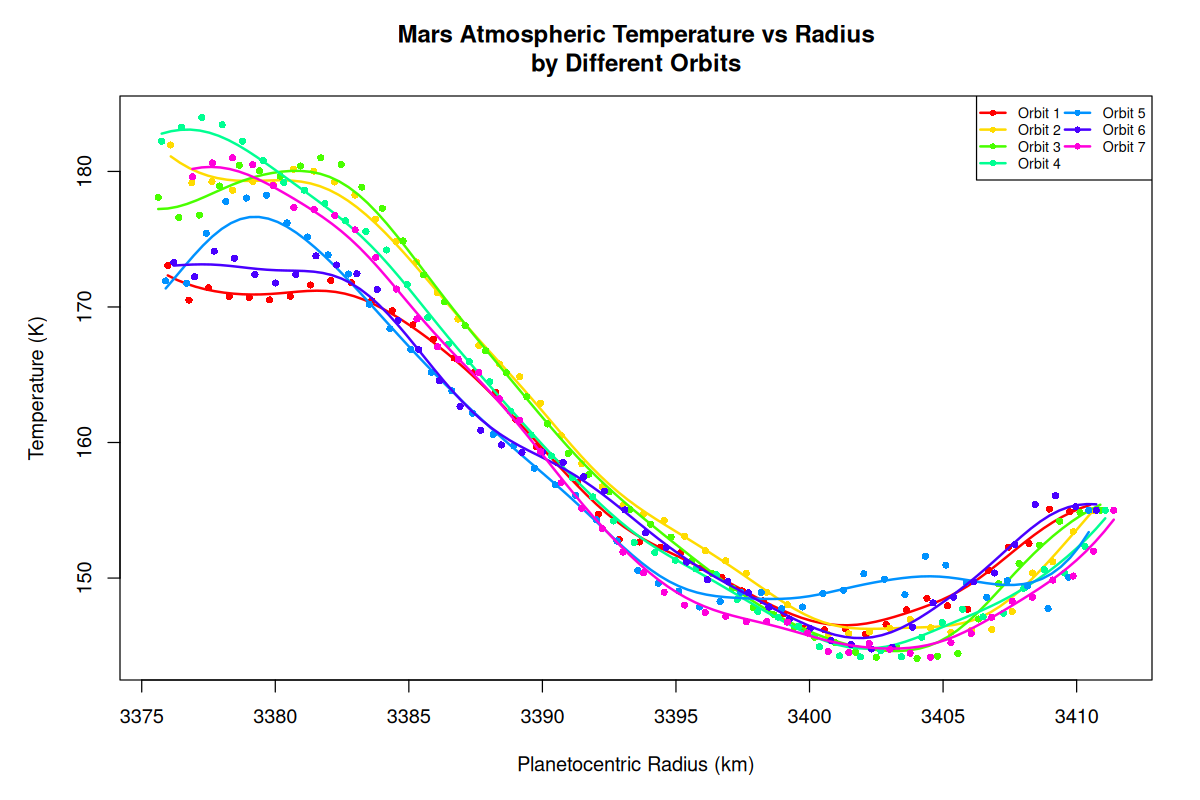
\includegraphics[width=0.85\textwidth]{exercise_04b_temp_vs_radius_by_orbit.png}
\caption{Nhiệt độ theo bán kính, phân theo 7 quỹ đạo}
\end{figure}

%=============================================================================
\subsection*{Phần (c): Xu hướng nhiệt độ theo áp suất}

Thay thế biến độc lập từ \texttt{radius} sang \texttt{pressure} và phân tích xu hướng.

\textbf{Kết quả:}
\begin{center}
\begin{tabular}{lcc}
\toprule
Bậc đa thức & Bandwidth $h$ (Pa) & CV Score \\
\midrule
$p=1$ (Local Linear) & 9.0585 & 6.8734 \\
$p=2$ (Local Quadratic) & 14.2685 & 6.7643 \\
\bottomrule
\end{tabular}
\end{center}

\textbf{Phân tích xu hướng:}

Kết quả cho thấy nhiệt độ \textbf{tăng} khi áp suất \textbf{tăng}:
\begin{align}
\frac{\partial \hat{m}(x)}{\partial x} \approx +0.032 \text{ K/Pa}
\end{align}

\textbf{Giải thích:}
\begin{itemize}
    \item Áp suất cao $\Rightarrow$ độ cao thấp (gần bề mặt) $\Rightarrow$ nhiệt độ cao
    \item Áp suất thấp $\Rightarrow$ độ cao lớn $\Rightarrow$ nhiệt độ thấp
    \item Quan hệ này \textbf{ngược lại} với phần (a)
\end{itemize}

Mối quan hệ này được giải thích bởi công thức áp suất khí quyển:
\begin{align}
P(z) \approx P_0 \exp\left(-\frac{z}{H}\right),
\end{align}
trong đó $z$ là độ cao và $H$ là scale height. Do áp suất giảm theo hàm mũ với độ cao, nên $T$ tăng theo $P$ tương đương với $T$ giảm theo độ cao.

\begin{figure}[h]
\centering
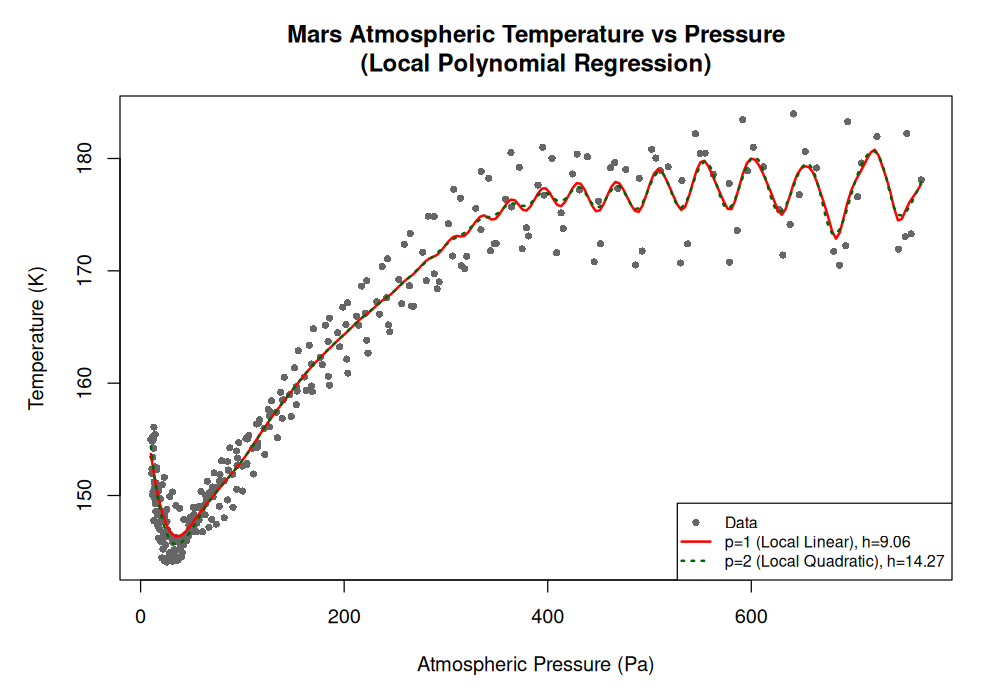
\includegraphics[width=0.8\textwidth]{exercise_04c_temp_vs_pressure.png}
\caption{Nhiệt độ khí quyển sao Hỏa theo áp suất}
\end{figure}

%=============================================================================
\subsection*{Tổng kết}

\begin{figure}[h]
\centering
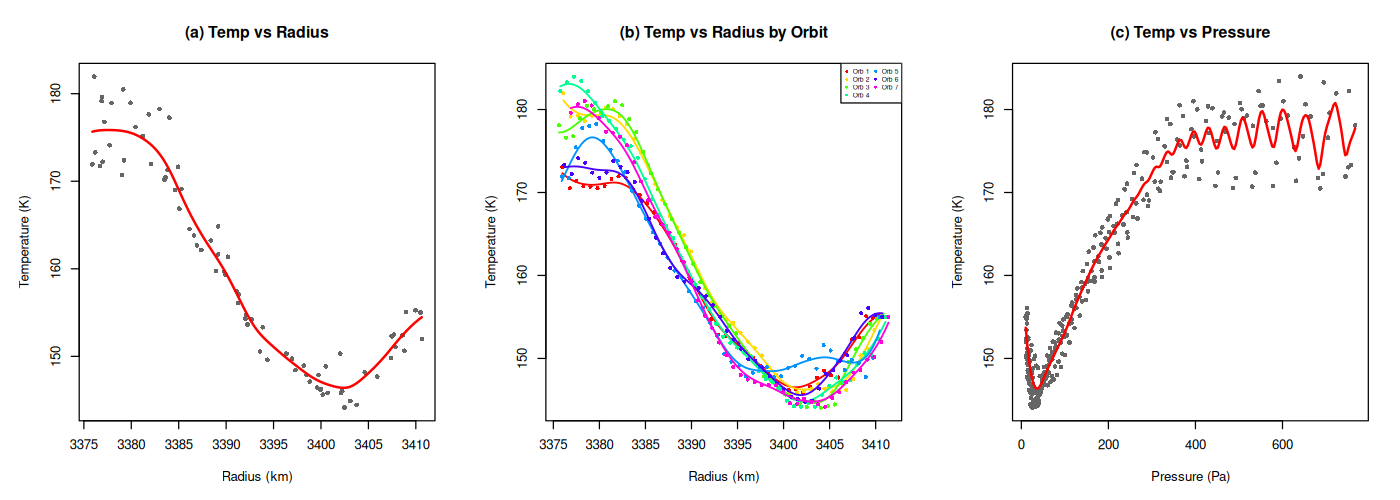
\includegraphics[width=\textwidth]{exercise_04_combined.png}
\caption{Tổng hợp kết quả phân tích: (a) Temp vs Radius, (b) Theo quỹ đạo, (c) Temp vs Pressure}
\end{figure}

\begin{center}
\begin{tabular}{lccc}
\toprule
Phần & Biến độc lập & Xu hướng & Độ dốc \\
\midrule
(a) & Radius & Giảm & $-0.61$ K/km \\
(b) & Radius (theo orbit) & Giảm (tất cả) & $-0.49$ đến $-0.76$ K/km \\
(c) & Pressure & Tăng & $+0.032$ K/Pa \\
\bottomrule
\end{tabular}
\end{center}

\textbf{Kết luận:}
\begin{enumerate}
    \item Nhiệt độ khí quyển sao Hỏa \textbf{giảm} khi bán kính (độ cao) tăng.
    \item Xu hướng này được xác nhận qua cả 7 quỹ đạo riêng biệt.
    \item Khi thay radius bằng pressure, xu hướng \textbf{ngược lại}: nhiệt độ tăng theo áp suất.
    \item Dữ liệu từ Mars Global Surveyor 2003 phù hợp với mô hình khí quyển hành tinh.
\end{enumerate}

\textbf{Code R:}
\begin{itemize}
    \item \texttt{exercise\_04.R}: Script phân tích chính
    \item \texttt{exercise\_04.Rmd}: R Markdown với phân tích từng bước
\end{itemize}

\end{giai}
\end{document}
